\section{Results}
\label{sec:results}

\Cref{tab:base} reports every base model under the three training distributions and \cref{fig:base} shows the same macro-F1 values with their confidence intervals.
\Cref{tab:ensembles} reports the ensembles and \cref{tab:groups} breaks recall down by head, middle and tail classes.

\begin{table*}[t]
  \centering
  \caption{Test accuracy and macro-F1 (\%) of the base models; brackets give 95\% bootstrap intervals for macro-F1. All rows are scored on the same 2{,}400 balanced test images. The weighted-CE rows train on the long-tailed set with inverse-frequency class weights.}
  \label{tab:base}
  \begin{tabular}{@{}lcccccc@{}}
    \toprule
    & \multicolumn{2}{c}{Balanced} & \multicolumn{2}{c}{Long-tailed} & \multicolumn{2}{c}{Rebalanced} \\
    \cmidrule(lr){2-3}\cmidrule(lr){4-5}\cmidrule(l){6-7}
    Model & Acc. & Macro-F1 & Acc. & Macro-F1 & Acc. & Macro-F1 \\
    \midrule
    \inputrows{tables/base.tex}
    \bottomrule
  \end{tabular}
\end{table*}

\begin{figure}[t]
  \centering
  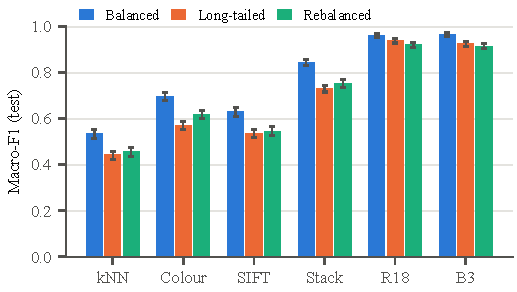
\includegraphics[width=\columnwidth]{figs/base_f1.pdf}
  \caption{CNNs lose 2.4--4.0\pp of macro-F1 under the long tail, hand-crafted pipelines 9--13\pp; rebalancing by augmentation helps only the latter. Bars show test macro-F1 of each base model under the three training sets, whiskers 95\% bootstrap intervals.}
  \label{fig:base}
\end{figure}

\subsection{Balanced training}
\label{sec:res_base}
The two families are far apart.
The single hand-crafted pipelines reach 53.3\% (LBP + \knn), 62.9\% (SIFT-BoW + SVM) and 69.8\% (colour histogram + SVM) macro-F1, and stacking their three descriptors raises this to 84.4\%.
Both CNNs exceed 96\%: \rn reaches 96.2\% and \eb 96.5\%, a difference that is not significant (McNemar $p=0.63$; 57 test images are classified correctly only by \eb and 51 only by \rn).
The confusion matrices in \cref{fig:confusion} locate the remaining hand-crafted errors among classes with similar texture, most often \emph{Highway} predicted as \emph{Railway} (11\% of \emph{Highway} images) and \emph{Lake} as \emph{River} (9\%), whereas \eb makes no off-diagonal error above 5\% of a class.

\begin{figure*}[t]
  \centering
  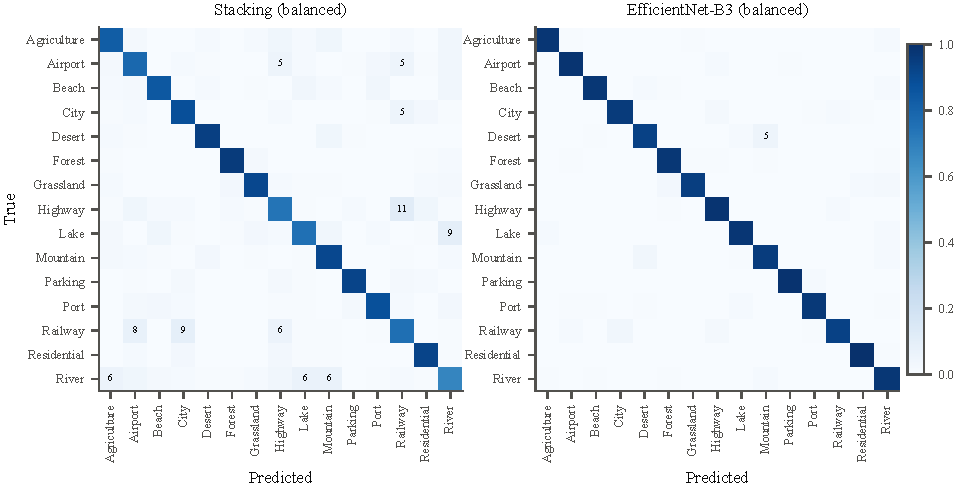
\includegraphics[width=0.86\textwidth]{figs/confusion.pdf}
  \caption{Hand-crafted errors concentrate on texture-similar classes. Row-normalised test confusion matrices after balanced training for stacking (left) and \eb (right); off-diagonal cells of at least 5\% are annotated.}
  \label{fig:confusion}
\end{figure*}

\subsection{Long-tailed training and rebalancing}
\label{sec:res_imbalance}
Training on the long-tailed set lowers every model significantly ($p<10^{-4}$ for each base model, McNemar against its balanced counterpart), but by very different amounts.
Macro-F1 falls by 9.1 to 12.9\pp for the hand-crafted pipelines and by 11.3\pp for stacking, against 2.4\pp for \rn and 4.0\pp for \eb (\cref{tab:base}).
Under the long tail \rn is the stronger network (93.8\% vs.\ 92.5\%, $p=0.017$).

\Cref{tab:groups} shows where the loss occurs.
Head-class recall is unchanged or slightly higher than under balanced training, consistent with the shifted class prior favouring the head, while tail-class recall falls from 82.8\% to 53.5\% for stacking and by about 8 and 11\pp for \rn and \eb.
The rarest class is the extreme case (\cref{fig:recall}): with 34 training images, stacking recognises 2.5\% of the \emph{River} test images, \rn 70.0\% and \eb 76.9\%.

\begin{table*}[t]
  \centering
  \caption{Mean test recall (\%) over the five head (544--374 long-tailed training images), middle (340--204) and tail (170--34) classes.}
  \label{tab:groups}
  \begin{tabular}{@{}lccccccccc@{}}
    \toprule
    & \multicolumn{3}{c}{Balanced} & \multicolumn{3}{c}{Long-tailed} & \multicolumn{3}{c}{Rebalanced} \\
    \cmidrule(lr){2-4}\cmidrule(lr){5-7}\cmidrule(l){8-10}
    Model & Head & Mid. & Tail & Head & Mid. & Tail & Head & Mid. & Tail \\
    \midrule
    \inputrows{tables/groups.tex}
    \bottomrule
  \end{tabular}
\end{table*}

\begin{figure*}[t]
  \centering
  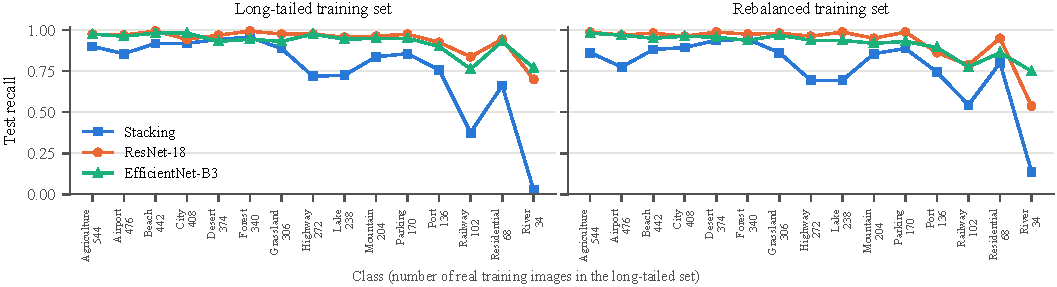
\includegraphics[width=\textwidth]{figs/per_class_recall.pdf}
  \caption{Recall collapses on the rarest classes for stacking, and augmentation-based rebalancing does not restore the CNNs' tail recall. Per-class test recall after long-tailed (left) and rebalanced (right) training; classes are ordered by their number of real training images.}
  \label{fig:recall}
\end{figure*}

Offline augmentation of the minority classes affects the two families in opposite directions.
For the hand-crafted pipelines it recovers part of the loss: colour-histogram SVM gains 5.0\pp ($p<10^{-4}$), LBP + \knn 1.4\pp ($p=0.049$), and SIFT-BoW and stacking gain 1.0 and 2.3\pp without reaching significance ($p=0.33$ and $0.14$); stacking's tail recall rises from 53.5\% to 62.2\%.
For the CNNs it is harmful: macro-F1 falls by 1.7\pp for \rn ($p=0.003$) and 1.1\pp for \eb ($p=0.029$), and their tail recall falls further, to 82.5\% and 84.2\%.
\emph{River} recall of \rn drops from 70.0\% to 53.7\%.
Re-weighting the loss instead of augmenting the data improves both networks over plain long-tailed training, to 95.0\% macro-F1 for \rn ($+1.2$\pp, $p=0.003$) and 93.4\% for \eb ($+0.9$\pp, $p=0.006$), mainly through the tail classes (91.5\% and 89.8\% tail recall).

\subsection{Ensembles}
\label{sec:res_ensembles}
Averaging the two CNNs is the only combination that improves on its best member in every setting (\cref{tab:ensembles}).
The \rn + \eb soft vote reaches 98.0\%, 95.3\% and 94.1\% macro-F1 on the balanced, long-tailed and rebalanced sets, gains of 1.5, 1.5 and 2.0\pp over the better network ($p<10^{-4}$ in each case).
On the balanced test set it corrects 48 images that \eb gets wrong while introducing 11 new errors.

Adding hand-crafted members does not help.
Pairing a CNN with \knn or stacking leaves the CNN's score unchanged or lowers it; under the long tail the \knn pairs lose 1.2 and 1.5\pp ($p<10^{-4}$).
The four-member ensemble of \knn, stacking and both CNNs gains 0.9\pp on the balanced and rebalanced sets but remains below the two-CNN vote, and the six-member ensemble is never significantly better than its best member and is 1.9\pp worse than \rn under the long tail ($p<10^{-3}$).
Hard voting is close to soft voting for two members, where our tie-breaking reduces it to a probability comparison, but falls well behind once four weak voters can outvote the two CNNs (88.6\% vs.\ 92.0\% for all six members under the long tail).
For reference, applying the first-member tie-break instead reproduces the first member's scores exactly for every two-member ensemble in \cref{tab:ensembles}.

\begin{table*}[t]
  \centering
  \caption{Macro-F1 (\%) of hard and soft voting ensembles and the change of the soft vote relative to its best member ($\Delta$, percentage points); $^\ast$ marks a significant difference (McNemar, $p<0.05$). R18: \rn, B3: \eb, Stack: stacking ensemble.}
  \label{tab:ensembles}
  \begin{tabular}{@{}lccccccccc@{}}
    \toprule
    & \multicolumn{3}{c}{Balanced} & \multicolumn{3}{c}{Long-tailed} & \multicolumn{3}{c}{Rebalanced} \\
    \cmidrule(lr){2-4}\cmidrule(lr){5-7}\cmidrule(l){8-10}
    Members & Hard & Soft & $\Delta$ & Hard & Soft & $\Delta$ & Hard & Soft & $\Delta$ \\
    \midrule
    \inputrows{tables/ensembles.tex}
    \bottomrule
  \end{tabular}
\end{table*}

The pairwise $Q$-statistics (\cref{eq:q}) show that the helpful pair is not the most diverse one.
\rn and \eb have the highest $Q$ in every setting (0.93, 0.90 and 0.86), i.e.\ they tend to fail on the same images, while pairs of a CNN and a hand-crafted model have $Q$ between 0.55 and 0.86.
The oracle accuracy of the six-member ensemble (99.2\% on the balanced set) shows that the weak members do contribute correct answers that the CNNs miss, but a fixed voting rule cannot pick them out from the many images on which the weak members are wrong and the CNNs are right.

\subsection{Grad-CAM case study}
\label{sec:res_gradcam}
The most frequent confusion of \rn after long-tailed training is \emph{Railway} predicted as \emph{Airport} (9 test images; \eb makes the same error on 7).
\Cref{fig:gradcam} shows a correctly classified \emph{Railway} image and three of these errors.
On the correct image both networks attend to the fan of converging tracks.
In the first error \rn concentrates on a cluster of large roofs between the tracks and predicts \emph{Airport}, while \eb follows the track lines and is correct; in the third, both networks attend to a long straight corridor and predict \emph{Airport}.
These maps are consistent with the networks associating large paved structures and long linear strips with airports, a cue that railway scenes share; we did not test this interpretation further.

\begin{figure}[t]
  \centering
  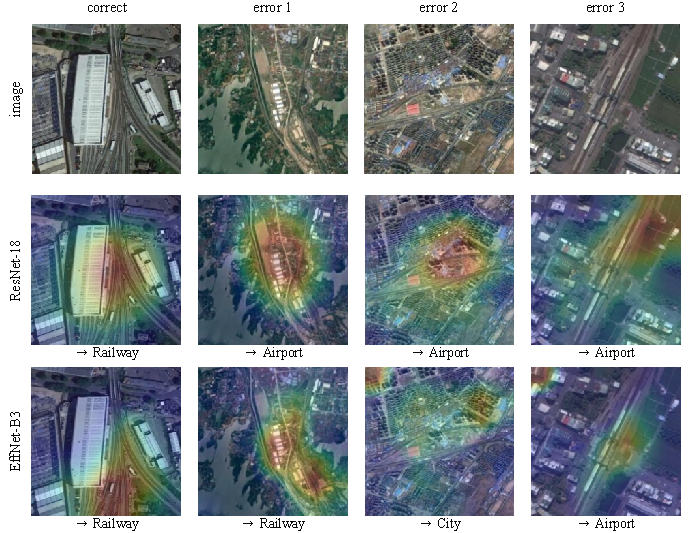
\includegraphics[width=\columnwidth]{figs/gradcam_longtail.pdf}
  \caption{When \rn mislabels \emph{Railway} as \emph{Airport}, its Grad-CAM focuses on large roofs or long straight strips rather than track fans. Test images (top) of the most frequent confusion after long-tailed training, with Grad-CAM maps for \rn (middle) and \eb (bottom); labels give each network's prediction.}
  \label{fig:gradcam}
\end{figure}
